This section presents an overview of search-based software test generation and automated crash reproduction and how they are connected to this thesis.

\subsection{Search-based Software Test Generation}
\label{sec:background:unit}

\begin{figure}
  \begin{center}
  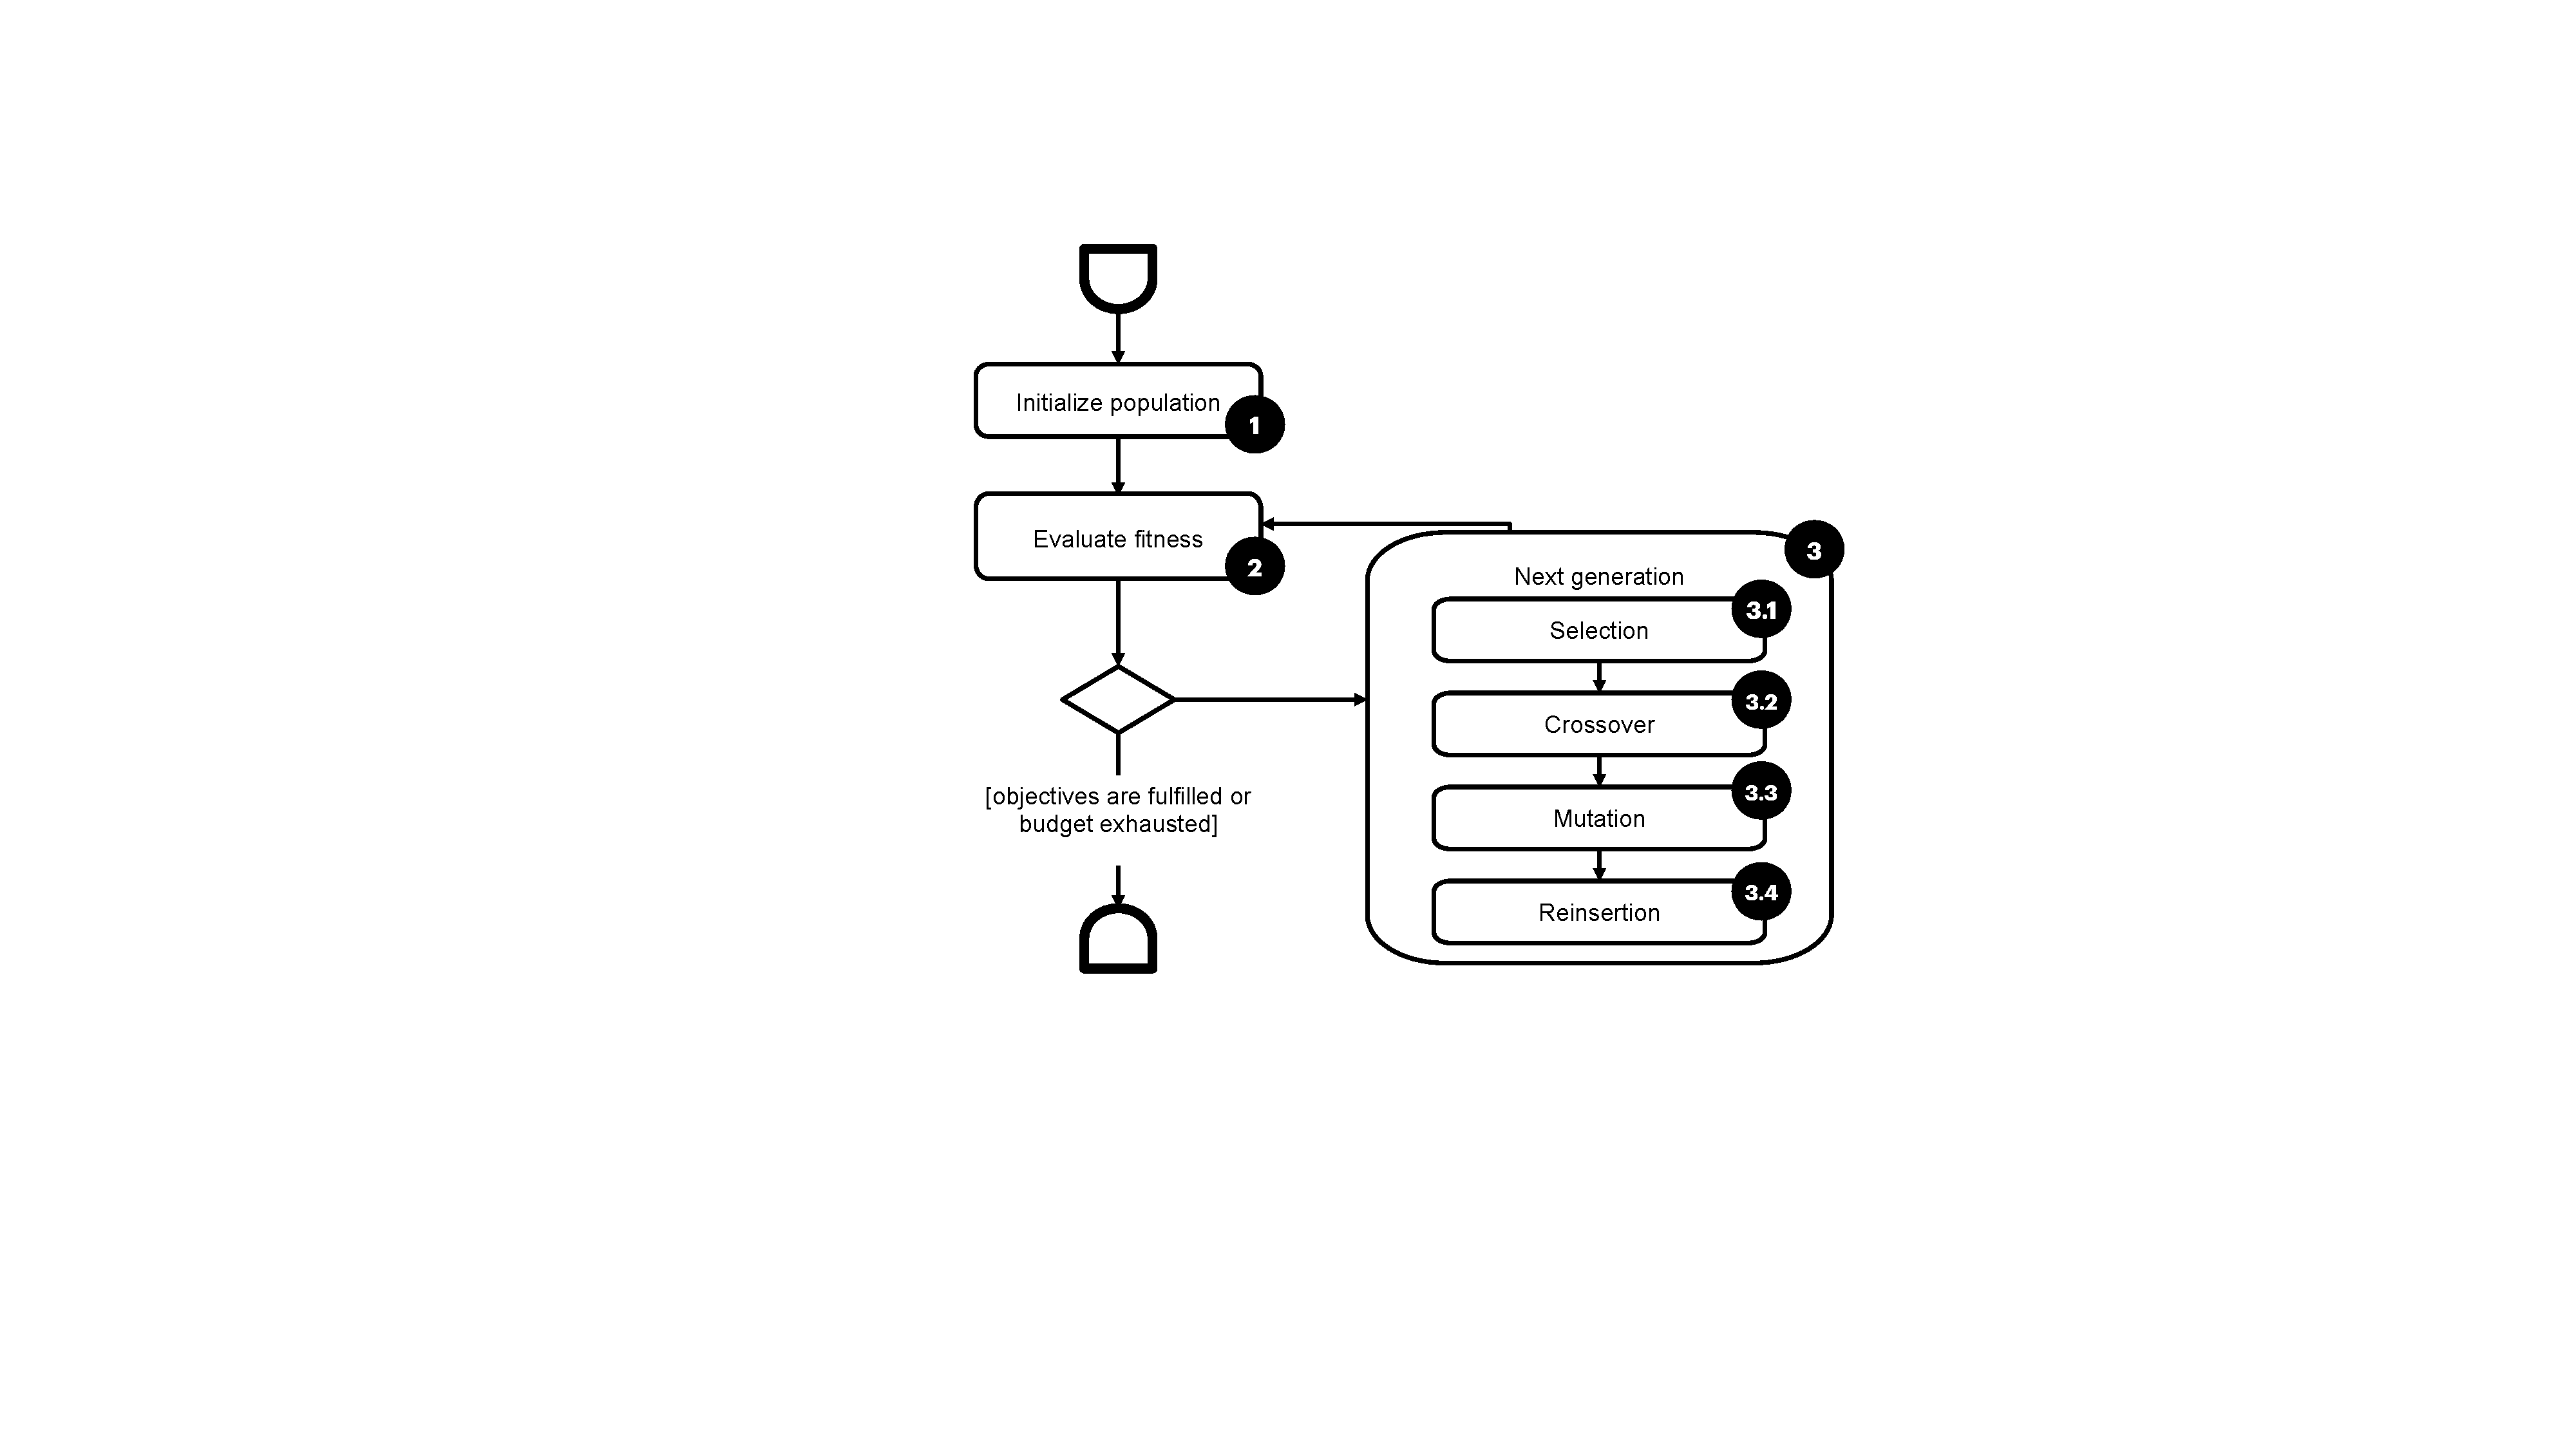
\includegraphics[height=3in]{figs/sb-test-generation.pdf}
\end{center}
  \caption{General overview of search-based test generation techniques using genetic algorithm.}
  \label{fig:sb-tg}
\end{figure}

McMinn~\cite{McMinn2004} defined search-based software testing (SBST) as \textit{``using a meta-heuristic optimizing search technique, such as a genetic algorithm, to automate or partially automate a testing task"}.
Within this realm, test data generation at different testing levels (such as \textit{unit testing}, \textit{integration testing}, \etc) has been actively investigated~\cite{McMinn2004}. This section 
provides an overview of earlier work in this area.

One of the most successfully used optimization techniques in search-based test generation is the genetic algorithm \cite{McMinn2011}. Figure \ref{fig:sb-tg} depicts how search-based test generation techniques uses genetic algorithm for test generation. 

In the first step, the algorithm generates a population of individuals. Each individual is either a single test case or test suite (a set of test cases). These individuals can be entirely randomly generated, or the algorithm can use seeding strategies in which it uses some information, such as hand-written tests, and generate tests using these existing data. Then, each generated individual is evaluated for fitness using one or multiple fitness functions (box 2 in Figure \ref{fig:sb-tg}). Next, it uses the fittest individuals (according to fitness function(s)) to generate the next population of individuals (box 3). 

For producing the next generation of individuals, first, the algorithm gets the individuals with the best fitness values (box 3.1 in Figure \ref{fig:sb-tg}). Then, it uses two genetic operators for generating new tests: \textit{Crossover} (box 3.2 in Figure \ref{fig:sb-tg}), which combines two selected individuals (parents) to create two new individuals (offsprings), and \textit{Mutation} (box 3.3 in Figure \ref{fig:sb-tg}), which add/remove/modify one or more statements in a selected test to generate a new one. Finally, the newly generated individuals are re-inserted into a new population (box 3.4 in Figure \ref{fig:sb-tg}).


The iteration between fitness evaluation (box 2 in Figure \ref{fig:sb-tg}) and producing the next generation (box 3 in Figure \ref{fig:sb-tg}) will continue until either the allocated budget is exhausted or all of the search objectives (represented as fitness functions) are fulfilled.

\subsubsection{Search-based approaches for unit testing}
Search-based software test generation algorithms have been extensively used for unit test generation. Previous studies confirmed that thus generated tests achieve a high code coverage~\cite{Panichella2018a, Campos2018}, real-bug detection~\cite{almasi2017industrial}, and debugging cost reduction~\cite{soltani2017, Panichella2016}, complementing hand-written tests. Also, a recent study by Panichella \etal \cite{panichella2020} verified that the unit tests generated by search-based test generation techniques have a low rate of test smell occurrence.

From McMinn's \cite{McMinn2004} survey about search-based test data generation, we observe that most of the current approaches rely on the control flow graph (CFG) to abstract the source code and represent possible execution flows. The $CFG_m=(N_m,E_m)$ represents a method\footnote{Or function in procedural programming languages.} $m$ as a directed graph of \textbf{basic blocks} of code (the nodes $N_m$), while $E_m$ is the set of the control flow edges. An edge connects a basic block $n_1$ to another one $n_2$ if the control may flow from the last statement of $n_1$ to the first statement of $n_2$. 

Listing~\ref{list:ClassA} presents the source code of \texttt{Person}, a class representing a person and her transportation habits. A \texttt{Person} can drive home (lines 4-10), or add energy to her car (lines~12-18). Figure~\ref{fig:CCFG} presents the CFG of two of Person's methods, with the labels of the nodes representing the line numbers in the code. Since method \texttt{driveToHome} calls method \texttt{addEnergy}, \texttt{node 6} is transformed to two nodes, which are connected to the entry and exit point of the called method. This transformation is explained in the last paragraph of this section.  

\begin{lstlisting}[frame=tb,
    caption={Class \texttt{Person}},
    label=list:ClassA,
    language=java,
    captionpos=t,
    numbers=left,
    belowskip=-2.5em,
    float=t,
    firstnumber=1]
class Person{
    private Car car = new Car();
    protected boolean lazy = false;
    public void driveToHome(){
        if (car.fuelAmount < 100) {
            addEnergy();
        } else {
            car.drive();
        }   
    }

    protected void addEnergy(){
        if (this.lazy) {
            takeBus();
        } else {
            car.refuel();
        }
    }   
  }
  \end{lstlisting}

  \begin{figure}[t]
    \centering
	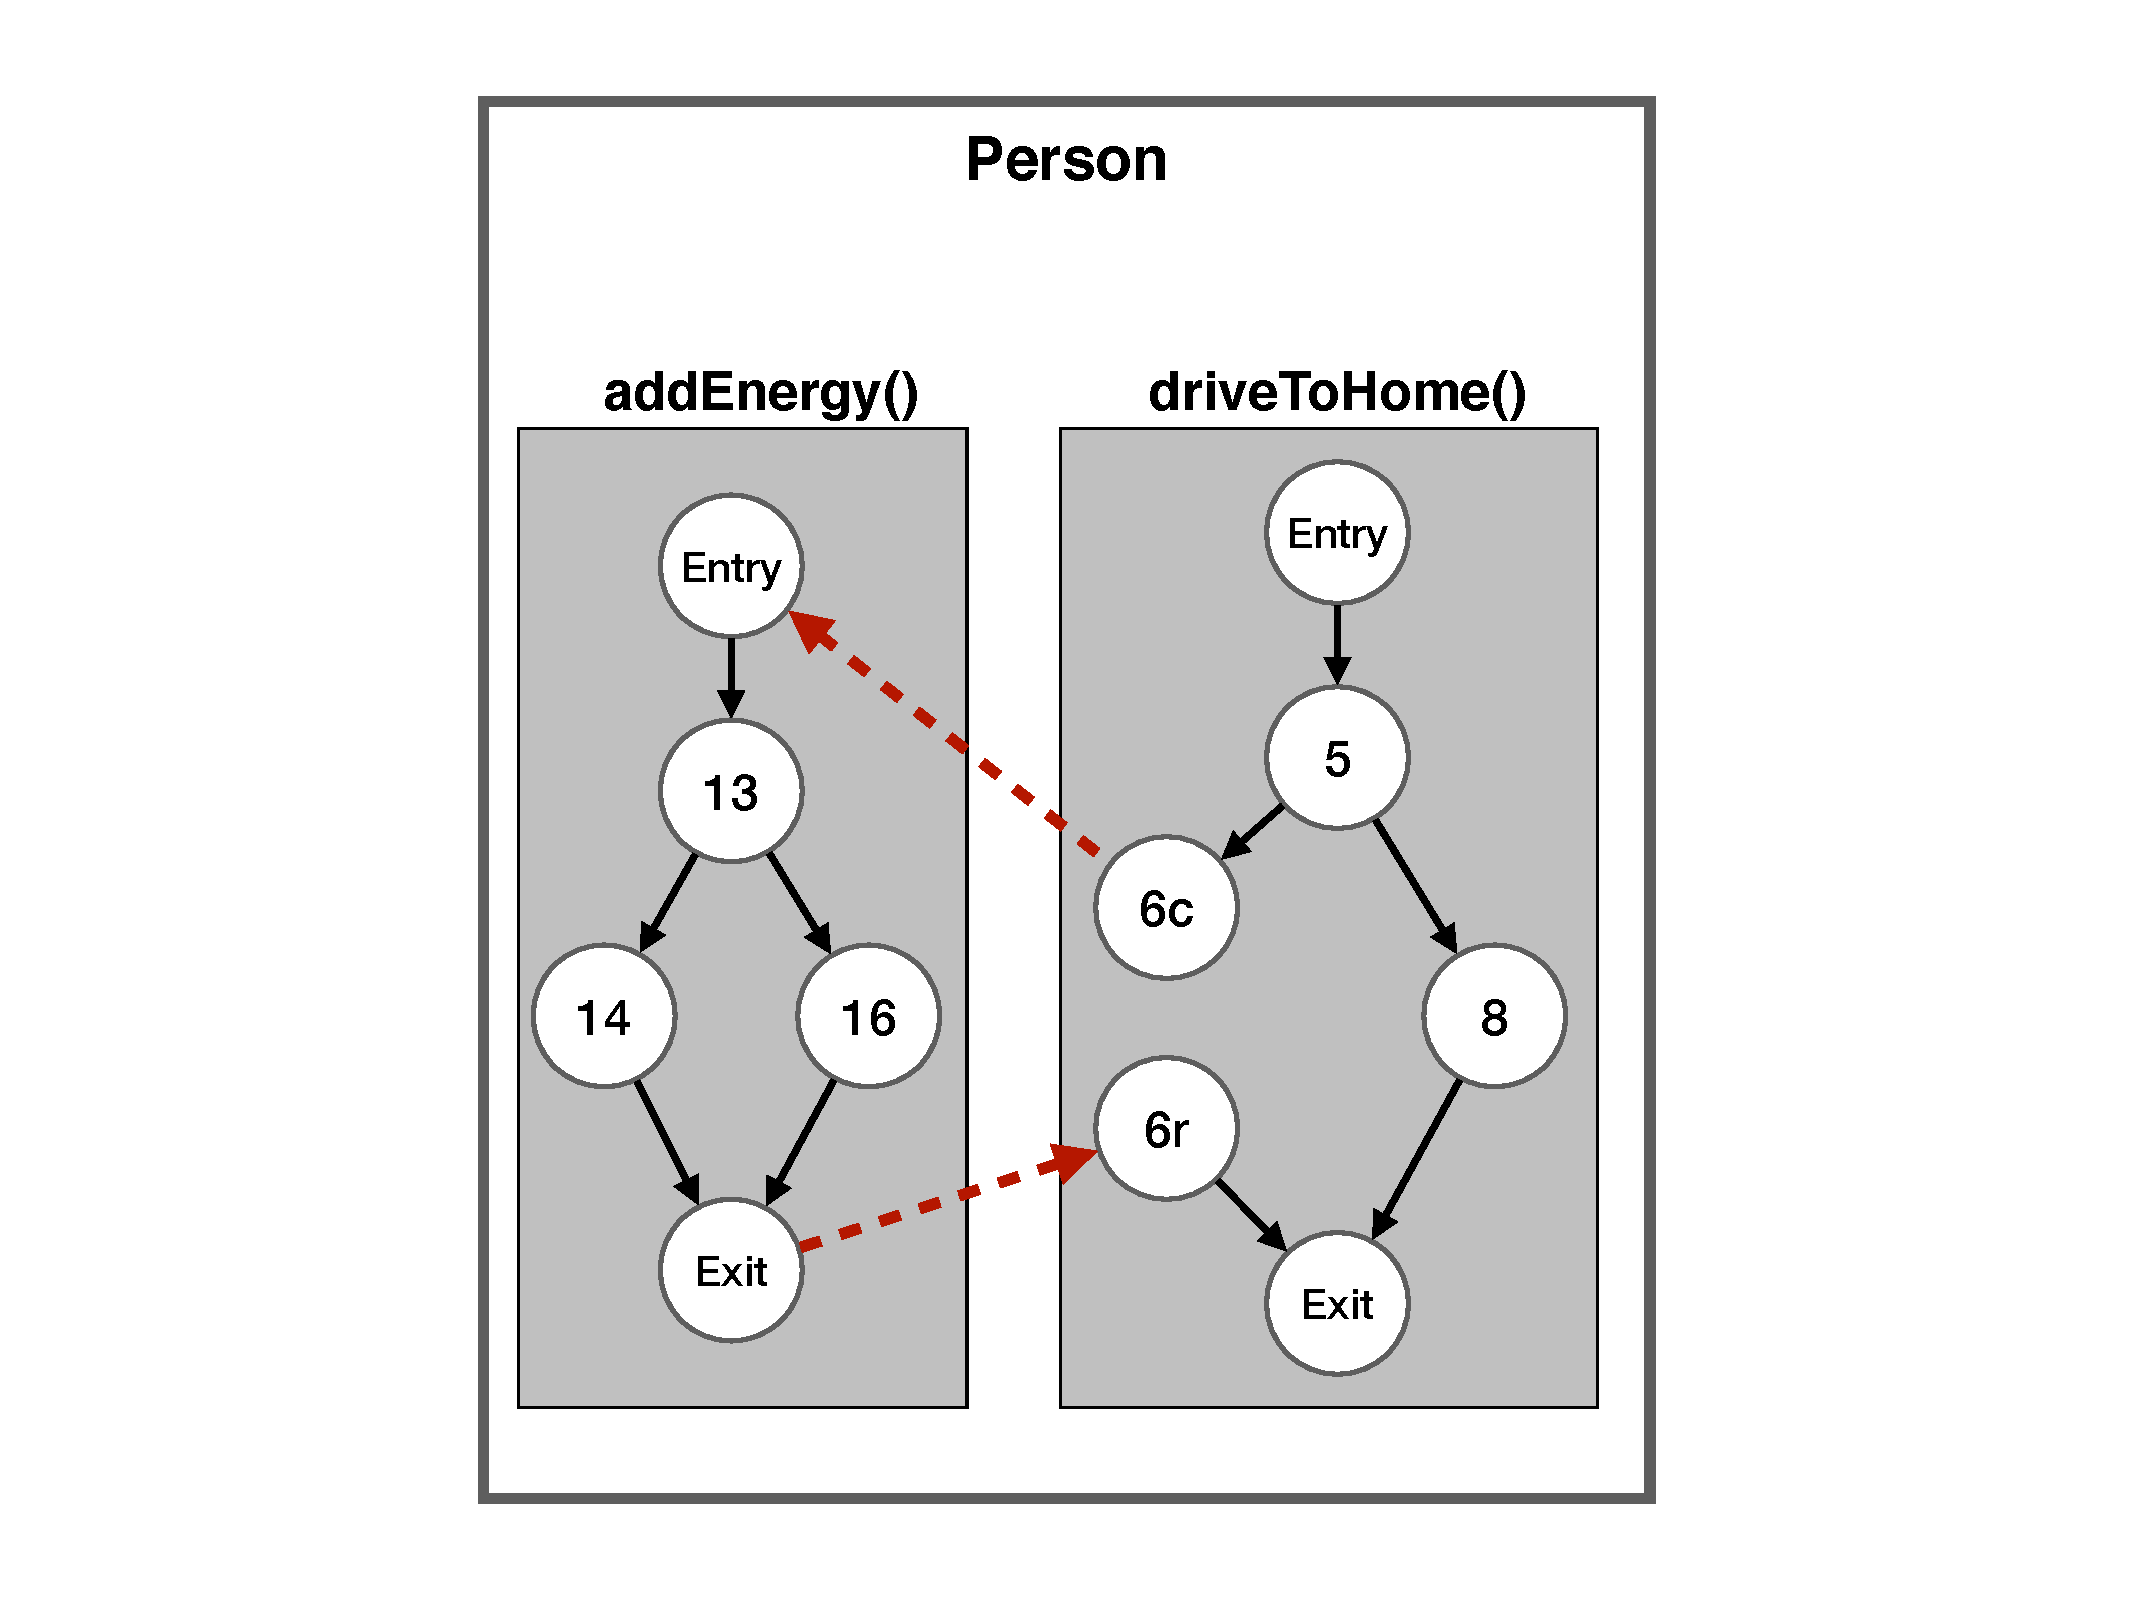
\includegraphics[width=0.85\linewidth]{figs/CCFG_new}
	\caption{Class-level CFG for class \texttt{Person}}
  \label{fig:CCFG}
\end{figure}


Many structural-based approaches combine two common heuristics to reach a high branch and statement coverage in unit-level testing. These two heuristics  are \textit{approach level} and \textit{branch distance}.
The \textit{branch distance} measures (based on a set of rules) the distance to \textit{satisfying} (true branch) and the distance to \textit{not satisfying} (false branch) a particular branching node in the program.
The \textit{approach level} measures the distance between the execution path and a target node in a CFG. To describe how this heuristic measures this distance, we 
rely on the concepts of \textbf{post-dominance} and \textbf{control dependency}~\cite{Allen:1970:CFA:800028.808479}. A \textit{node A} is control dependent on \textit{node B} in a control flow graph if \textit{node B} contains a branch, which can change the execution path away from reaching \textit{node A}.

%
As an example, in Figure \ref{fig:CCFG}, \textit{node 8} is control dependent on \textit{node 5} and \textit{node 8} post-dominates edge $\langle 5,8\rangle$. %, but it does not post-dominate $node 5$ itself ($node 5$ can reach the exit point through $node 6$). 
The \textit{approach level} is the minimum number of control dependencies between a target node and an executed path by a test case. 

One of the best tools for performing search-based test generation is \evosuite \cite{panichella2020evosuite}. This tool gets a Java application and one of its classes as a class under test. Then, it starts a genetic algorithm to generate a test suite fulfilling different testing criteria for the given class. This tool contains multiple  genetic algorithms \cite{fraser2012whole,Panichella2018}. Also, it can generate tests according to various criteria such as line coverage, branch coverage, weak mutation, \etc

This thesis leverages the information carved from different sources (\eg hand-written tests, source code, \etc) to introduce search objectives complementing approach level and branch distance for different test generation scenarios. 
% Chapters \ref{sec:jcrashpack:introduction} to \ref{section:bbc:introduction} try to achieve this goal in test generation for on instance of specific behaviors (\ie crash reproduction). Chapter \ref{sec:cling:introduction} uses the call-site information to generate test cases for class integration. Finally, 

\subsubsection{Search-based approaches for integration testing}

Search-based approaches are widely used for test ordering \cite{Wang2010, Steindl2012, Hashim2005, Vergilio2012, Bansal2009, JIiang2019, Borner2009, Mariani2016, Guizzo2015, Abdurazik2009, DaVeigaCabral2010, Briand2003a, Vergilio2012}, typically with the aim of executing those tests with the highest likelihood of failing earlier on. % These studies propose a solution for ordering the integration testing of the classes in the software under test (SUT). However, they do not offer any solution for automated integration test generation.
However, to the best of our knowledge, search-based approaches have rarely been used for generating integration tests. Ali Khan \etal \cite{AliKhan2013} have proposed a high-level evolutionary approach that detects coupling paths in data-flow graphs of classes and generates tests for the detected coupling paths. Moreover, they proposed another approach for the same goal, which uses Particle Swarm Optimization \cite{Khan2014}. However, the paper does not describe the fitness function and genetic algorithm used in their approach, nor any evaluation for examining the quality of the tests generated by this approach. 
The paper also does not check whether the tests can complement tests generated by existing search-based unit testing approaches. Besides, since objectives are defined according to the \textit{def-use} paths between classes, the number of search objectives can grow exponentially, thus severely limiting the scalability of the approach.

In Chapter \ref{sec:cling:introduction} we propose a novel approach for class integration test generation.
Instead of using the data flow graph, which is relatively expensive to construct as it needs to find the coupling paths, we use the information available about the the integration between classes to calculate the fitness of the generated tests.
\subsubsection{Search-based approaches for other testing levels}

Arcuri \cite{Arcuri2019} proposed EvoMaster, an evolutionary-based white-box approach for system-level test generation for RESTful APIs. A test for a RESTful web service is a sequence of HTTP requests. EvoMaster tries to cover three types of targets:
 \begin{inparaenum}[(i)]
 \item all of the statements in the System Under Test (SUT);
 \item all of the branches in the SUT; and
\item different returned HTTP status codes.
\end{inparaenum}
Although EvoMaster tests different classes in the SUT, it does not systematically target different integration scenarios between classes.

In contrast to EvoMaster, other approaches perform fuzzing \cite{Holler2012}, \textit{``an automated technique providing random data as input to a software system in the hope to expose a vulnerability.''} Fuzzing uses information like grammar specifications \cite{Holler2012, beyene2012, coppit2005, godefroid2008} or feedback from the program during the execution of tests \cite{Padhye2019} to steer the test generation process.
These fuzzing approaches generate only input data but do not generate a full test case.

The approaches introduced in this thesis perform white-box testing.

\subsection{Search-based Crash Reproduction \protect\footnote{ This section is partly based on \faFileTextO~\emph{B. Cherry, X. Devroey, P. Derakhshanfar, and B. Vanderose. Crash reproduction difficulty, an initial assessment, BENEVOL'20} \cite{Cherry2020a}}}

Another application of search-based test generation techniques is in \textbf{automated crash reproduction}. 
Information about a software crash, like a \textit{stack trace} for Java applications, are usually reported to the developers through an issue tracker. Based on the report's information, the developers debug the software by identifying the crash's root cause and applying a fix to the code. To ease their investigation, developers can start their debugging process by \textit{reproducing} and \textit{exposing} the crash, and (latter) write a test case to ensure that the fix does not induce regression errors \cite{Zeller2009}. 
%
Recent developments lead to the (partial) automation of the crash reproduction and exposure process. When a new issue is created, an automated process fetches the stack trace and try to generate a \emph{crash reproducing test case} able to reproduce and expose the crash  \cite{Gagliardi2019}. Various approaches have been developed to automate the generation of a crash reproducing test case \cite{Nayrolles2017, Soltani2018a, Chen2015, Xuan2015}. Among those, search-based crash reproduction yields the best results by reproducing more crashes and generating helpful test cases \cite{Soltani2018a}. It has also been confirmed that crash reproducing test cases generated by this approach aid developers in fixing bugs \cite{Soltani2018a}.

\begin{lstlisting}[
        caption=XWIKI-13377 crash stack trace \cite{Derakhshanfar2020},
        label=lst:stacktrace-intro,
        numbers=left,
        firstnumber=0,
        float=t
        ]
java.lang.ClassCastException: [...]
    at [...].BaseStringProperty.setValue([...]:45) (*@\label{line:lowestframe}@*)
    at [...].PropertyClass.fromValue([...]:615) (*@\label{line:targetframe}@*)
    at [...].BaseClass.fromMap([...]:413)
    [...] 
\end{lstlisting}

Search-based crash reproduction takes as input the application in which the crash happened, and a stack trace (reported in a crash report) with one of its frames indicated as the \textit{target frame}. Then, it initiates a search process to generate a test case, which reproduced the given stack trace from the deepest frame up to the target frame. For instance, by passing the stack trace in Listing \ref{lst:stacktrace-intro} as the given tack trace and frame \ref{line:targetframe} as the target frame, search-based crash reproduction generates a test case which reproduces the first two frames of the given stack trace with the same type of exception (\texttt{ClassCastException}).


\subsubsection{Fitness function}

To reproduce a given crash, search-based crash reproduction relies on a fitness function called \WS (described in Equation \ref{eq:fitnessfunction1}) to evaluate the generated test cases, thereby guiding an evolutionary algorithm towards generating a crash reproducing test case for a given stack trace.
%
\begin{equation} \label{eq:fitnessfunction1}
f(t) = 
\left\{
\footnotesize
  \begin{array}{ll}
    3 \times d_{s}(t) + 2 \times max(d_{e}) + max(d_{t})  & \textit{line is not reached}\\
    2 \times d_{e}(t) + max(d_{t})   & \textit{line is reached}\\
    d_{t}(t)  & \textit{exception is thrown}
  \end{array}
\right.
\end{equation}
%
Where $d_{s}(t) \in [0,1]$  measures the distance between the execution of a generated test $t$ from reaching the line of the target frame (\textit{target line}) using the approach level and branch distance \cite{McMinn2004}; $d_{e}(t) \in \{0,1\}$ is a binary value indicating if  $t$ throws the same type of exception as the given stack trace ($d_{e}(t) = 0$) or not ($d_{e}(t) = 1$); $d_{t}(t) \in [0,1]$ compares the similarity of the frames in the given thrown stack trace by test $t$ against the frames in the given stack trace; and $max(.)$ indicates the maximum possible value for each heuristic.

Since considering $d_{e}(t)$ and $d_{t}(t)$ is only relevant if test $t$ covers the target line ($d_{s}(t) = 0$), \WS (first line of Equation \ref{eq:fitnessfunction1}) sets the maximum value for these two heuristics before achieving the target line coverage. Therefore, $f(t) \in ]3,6]$ before reaching the target line. Likewise, as shown by the second line of Equation \ref{eq:fitnessfunction1}, measuring the stack trace similarity ($d_{t}(t)$) is not relevant before fulfilling the exception coverage ($d_{e}(t)$), and thereby \WS  sets the maximum possible value for $d_{t}(t)$. Hence, $f(t) \in ]1,3]$ before $t$ throws the same type of exception as the given stack trace. Finally, when $d_{s}(t)$ and $d_{e}(t)$ are zero, $f(t) \in [0,1]$ according to the value of $d_{t}(t)$. Since the process is a minimization process, the three heuristics are equal to zero for a crash reproducing test case.

In this thesis, we have implemented a new open-source search-based crash reproduction framework called \botsing. This framework contains the previously introduced search-based crash reproduction approach (\eg \evocrash). Also, the novel techniques introduced in this thesis are all implemented in this framework.
